\documentclass[11pt,a4paper]{article}

\usepackage[utf8]{inputenc}
\usepackage[T1]{fontenc}
\usepackage{lmodern}
\usepackage{microtype}
\usepackage[margin=1in]{geometry}
\PassOptionsToPackage{hyphens}{url}
\usepackage{hyperref}
\usepackage{graphicx}
\usepackage{xcolor}

\setlength{\emergencystretch}{3em}
\widowpenalty=10000
\clubpenalty=10000

\hypersetup{
  colorlinks=true,
  linkcolor=black,
  citecolor=blue!50!black,
  urlcolor=blue!50!black,
  pdftitle={Agentic, Context-Aware Risk Intelligence in the Internet of Value --- a summary},
  pdfauthor={Basel Magableh; OmniRisk Research},
}

\title{Agentic, Context-Aware Risk Intelligence\\
       in the Internet of Value\\[0.4em]
       \large{\normalfont(a short summary)}}
\author{%
  Basel Magableh\textsuperscript{1,*} \quad\quad OmniRisk Research\textsuperscript{2} \\[0.8em]
  \normalsize\textsuperscript{1}School of Computer Science, Technological University Dublin, Ireland \\
  \normalsize\textsuperscript{2}Rayachain Lab, Dublin, Ireland \\[0.4em]
  \normalsize\textsuperscript{*}Correspondence: \texttt{basel.magableh@tudublin.ie}
}
\date{May 2026 \\ \textbf{v0.5 (draft, CEO read-through pending)}}

\begin{document}
\maketitle

\begin{abstract}
Token value moves across many chains, exchanges, and bridges. The risk
to a participant is now composite (route, sentiment, liquidity, and the
policy a system is willing to commit to), not a property of any one
chain. We argue this calls for a new kind of risk primitive built from
five engines, which include prediction, decentralised verification,
sentiment fusion, an agentic decision layer under written rules, and a
scenario engine that turns forecasts into pre-committed action programs.
We anchor the architecture in two public artefacts: a 27-hour on-chain
liquidity defence and a 168-hour production calibration arc.
\end{abstract}

\section*{The problem in one paragraph}

The Internet of Value is no longer one chain at a time. A single token
can live on Ethereum, on Solana, and on a half-dozen rollups, with
bridges connecting them and routing software choosing among them in
milliseconds. The risk a participant carries is composite: the route
they take, the venue they trade on, the narrative driving the moment,
and the policy they have committed an automated agent to follow.
Existing risk tools mostly think one chain at a time. They flag a
contract as risky, an address as sanctioned, a bridge as exploited ---
but they do not stitch the picture together. The question we ask is
simpler than it sounds: what does context-aware risk intelligence have
to do, and how is it kept honest?

\section*{The five engines}

The architecture composes five engines over a shared intelligence
fabric.

The \textbf{prediction engine} forecasts price, liquidity, volatility,
and route health. Think of it as the weather report --- point estimates
and probability distributions, run continuously. In production today on
a 30-day horizon over 21 anchor symbols, calibrated against 66{,}118
samples.

The \textbf{Bittensor verification subnet} decentralises the prediction
layer. A heterogeneous population of miners produces forecasts;
validators score them economically against realised outcomes. Think of
it as Wikipedia for forecasts --- competing contributors weighted by
reliability --- except the reward is TAO, not reputation.

The \textbf{sentiment-fusion engine} ingests text streams (news, social,
grey literature) and on-chain flow signals together. Twelve news
adapters and three social adapters feed it; outputs are fused late and
stacked. Think of it as a tape reader who also follows the chat.

The \textbf{agentic engine} is the LLM-mediated layer that selects and
executes actions under a written constitution: \emph{buy-only},
\emph{never use the deployer wallet}, \emph{live mode requires board
sign-off}. Paused by default; daily-cap raises require an explicit
out-of-band approval. Think of it as a paid trader with a written
mandate and a chaperone.

The \textbf{scenario engine} turns forecasts into pre-committed action
programs: \emph{if liquidity drops 20\% in the next hour, deploy 0.3
SOL of buy capacity to tier 3.} Programs are registered in advance and
executed within resource bounds. Think of it as a fire drill that runs
automatically when the alarm goes off.

\begin{figure}[h]
\centering
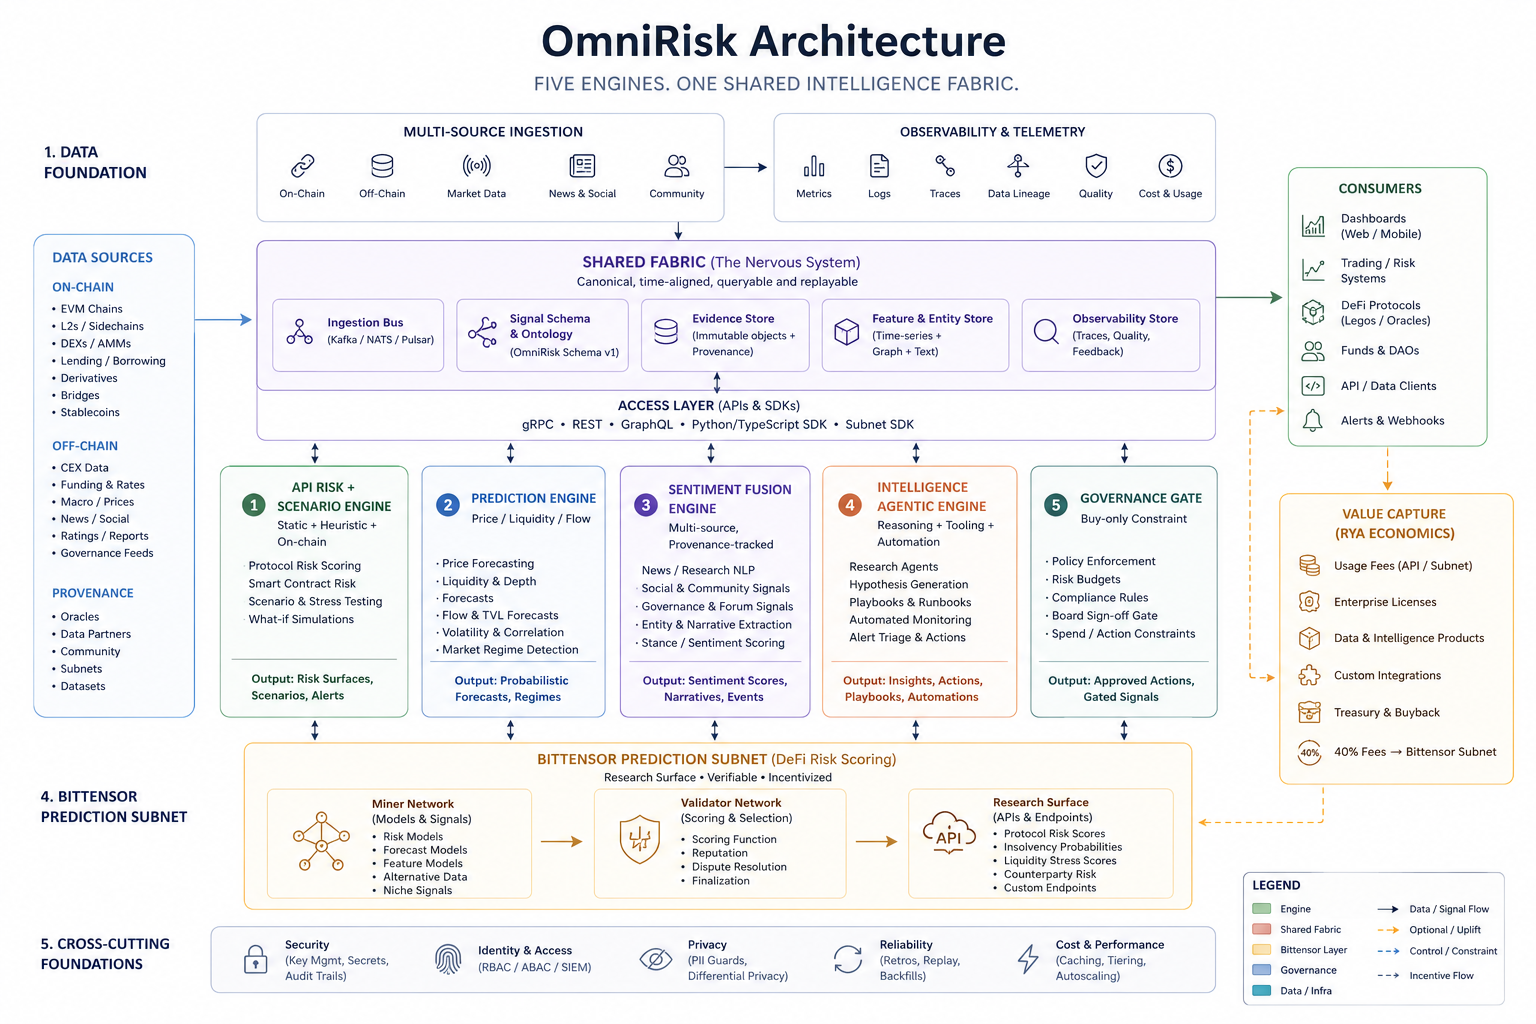
\includegraphics[width=\linewidth]{figures/omnirisk-architecture.png}
\caption{The OmniRisk architecture: five engines composed over a single
shared intelligence fabric. Multi-source ingestion (on-chain, off-chain,
market, news, community) and observability telemetry feed a canonical,
time-aligned, queryable signal layer. The five engines consume the
fabric in parallel; the agentic engine integrates them and is wrapped
by a governance gate (paused by default, board approval required to
flip live).}
\label{fig:summary-architecture}
\end{figure}

\section*{The case study (in plain English)}

On 2026-05-06 at 01:00~UTC, the protocol token \textsc{rya} was down
roughly 60.9\% over the previous day on its single Solana liquidity
pool. Pool depth had drifted from about \$6{,}098 to \$5{,}418 ---
small in absolute terms, large enough on a micro-cap pool that the next
sell would set the price for hours.

We had a deterministic Trader-role policy ready for exactly this case.
The CEO recorded an authorisation in the public issue thread, topped
the wallet up by 5~SOL, and four minutes later the bot fired its first
buy: 0.10~SOL, split across five 0.02~SOL slices over 150~seconds. A
second sign-off raised the daily cap from 1 to 3~SOL with a written
rationale.

Twenty-nine more buys followed at the bottom of a four-tier ladder. A
ratchet primitive raised the floor by 50 basis points twice --- once
when cumulative spend crossed 2~SOL, again at 4~SOL. By 06:13~UTC the
daily cap had bound at 3.000~SOL exactly. Price had climbed about 19.5\%
off the floor; pool liquidity had returned to baseline. A non-bot buyer
printed at the recovered level around 10:00~UTC.

That afternoon a second stress event: $-5.84\%$ in roughly an hour. A
third sign-off raised the cap from 3 to 5~SOL. Twenty-one more buys
completed across the date boundary. Then at 02:38~UTC the safety
circuit fired: a single sell drove price down 46\% in 3--10~minutes,
draining \$1{,}666 of liquidity. The bot auto-paused exactly as
configured. At 03:44~UTC the CEO recorded an explicit override; the
engine resumed at the new \$0.0000414 floor, and the stop-loss circuit
re-armed at the new baseline.

The price recovery is not the point. The point is that the constitution
held under two stop-loss events and three out-of-band approvals, and
that the entire decision chain --- every cap raise, every override,
every buy --- can be reconstructed from the public issue thread plus the
public decision log.

\section*{The 168-hour calibration arc}

The prediction engine has been running on the production deployment for
months. The number that matters is small and uncomfortable: on a broad
cohort, the live-API directional accuracy has hovered around 53\% ---
barely above chance. That is not a marketing number. It is the right
number to compare against.

On the freshest 168-hour evaluation, restricted to the top 1{,}000
assets by market capitalisation (a low base-rate cohort), accuracy
reaches 99.34\% on 915~samples. Stripped of the cohort restriction, the
comparison would not survive. Two things make this honest. First, on
this cohort a model that says ``no crash'' most of the time is right
almost by construction. Second, the metric that survives both class
imbalance and overconfidence is the Brier calibration error, which on
the same cohort lands at \textbf{0.1335} --- closer to perfect (0)
than to a coin flip (0.25), but well short of headline-grade.

\section*{What this isn't}

Three things to name directly.

This isn't a trading bot for retail. It is buy-only, capped per UTC
day, and gated by board sign-off. The ladder, the cooldown, the
stop-loss, the cap-raise approval path --- all of these only make sense
for a project's own protocol token where the operator is the wallet's
only counterparty. It would not work as a generic ``defend my coin''
product.

This isn't a decentralised system yet. The Bittensor verification
subnet is a testnet shadow deployment --- 5{,}097 successful rounds
and zero auth failures so far, which validates the orchestration path
but not the validator-loss claim. The economic verification has to
wait for a real metagraph.

This isn't a generalisation claim. One pool, one token, one 27-hour
cycle. Replication on other pools is the obvious next step.

\section*{Read more}

The full architecture, threat model, and formal validator-loss
specification live in the companion focused paper at
\path{papers/2026/agentic-iov-risk-focused/manuscript.tex} in the same
source repository. The buy-by-buy decision log for the case study is
published as a public article at
\url{https://paragraph.com/@rayachain/defending-rya-a-public-on-chain-liquidity-defence-playbook}.
Reproducibility data (prediction-router metrics CSV; Bittensor
shadow-validator soak telemetry) is committed alongside the focused
paper at git commits \texttt{b419338} and \texttt{e726153}. Reviewer
access to the live OmniRisk prediction-router endpoint can be requested
under NDA.

\end{document}
